\documentclass[../NormediProgetto.tex]{subfiles}

\begin{document}
	
	\chapter{Processi Organizzativi}
	
	\section{Scopo}
	Lo scopo di questo processo è fornire norme e strumenti per organizzare il lavoro del gruppo per il corretto svolgimento del progetto.
	
	\section {Descrizione}
	Durante questo processo sono trattati:
	\begin{itemize}
		\item Ruoli di progetto;
		\item Comunicazioni;
		\item Incontri;
		\item Strumenti di coordinamento;
		\item Strumenti di versionamento.
		
	\end{itemize}
	
	\section {Ruoli di progetto}
	
	Ogni ruolo viene ricoperto da ciascun componente del gruppo a turno, dando la possibilità ad ogni membro di fare esperienza in ognuno di essi. L'organizzazione e la pianificazione delle attività da svolgere in ogni ruolo è regolata dal PP. La descrizione dei ruoli viene approfondita nelle sezioni seguenti.
	
	\subsection {Amministratore di progetto}
	
	L’\textit{Amministratore di Progetto} deve controllare e amministrare tutto l’ambiente di lavoro con piena responsabilità sulla capacità operativa e sull’efficienza. 
	\\ \noindent Le sue mansioni sono: 
	
	\begin{itemize}
		\item ricerca di strumenti che migliorino l’ambiente di lavoro e che lo automatizzino ove possibile;
		\item gestione del versionamento;
		\item controllo di versioni e configurazioni del prodotto software; 
		\item risoluzione dei problemi di gestione dei processi; 
		\item controllo della \glossario{qualità}{qualita} sul prodotto.
	\end{itemize}
	
	\subsection {Responsabile di progetto}
	
	Il \textit{Responsabile di Progetto} è il punto di riferimento sia per il \glossario{committente}{committente} che per il \textit{fornitore}. Esso deve anche approvare le scelte prese dal gruppo e se ne assume la responsabilità. 
	\\ \noindent Le sue mansioni sono:
	
	\begin{itemize}
		\item coordinare e pianificare le attività di progetto;
		\item approvare la documentazione;
		\item effettuare uno studio e gestire in modo corretto i rischi;
		\item approvare l'offerta economica;
		\item gestire le risorse umane distribuendo in modo corretto i carichi di lavoro.
	\end{itemize}
	
	\subsection {Analista}
	
	L'\textit{Analista} si occupa dell'analisi dei problemi e del dominio applicativo. Normalmente questo ruolo non rimane attivo per tutta la durata del progetto, bensì concentra tutta la propria attività nelle fasi iniziali.
	\\ \noindent Le sue principali mansioni sono:
	
	\begin{itemize}
		\item comprensione del problema e della sua complessità;
		\item produzione dello \textit{Studio di Fattibilità} e dell'\textit{Analisi dei Requisiti}.
	\end{itemize}
	
	\subsection {Progettista}
	
	Il \textit{Progettista} gestisce gli aspetti tecnologici e tecnici del progetto.
	\\ \noindent Le sue mansioni sono:
	
	\begin{itemize}
		\item rendere facilmente mantenibile il progetto;
		\item effettuare scelte efficienti ed ottimizzate su aspetti tecnici del progetto.
	\end{itemize}
	
	\subsection {Verificatore}
	
	Il \textit{Verificatore} deve garantire una verifica completa ed esaustiva del progetto basandosi sulle solide conoscenze delle sue normative.
	\\ \noindent Le sue mansioni sono:
	\begin{itemize}
		\item controllare le attività del progetto secondo le normative prestabilite.
	\end{itemize}
	
	\subsection {Programmatore}
	
	Il \textit{Programmatore} è il responsabile della codifica del progetto e delle componenti di supporto, che serviranno per effettuare le prove di verifica e validazione sul prodotto.
	\\ \noindent Le sue mansioni sono:
	
	\begin{itemize}
		\item versionamento del codice prodotto;
		\item implementare le decisioni del \textit{Progettista};
		\item realizzazione degli strumenti per la verifica e la validazione del software;
		\item scrittura di un codice pulito e facile da mantenere, che rispetti le \textit{Norme di Progetto}.
	\end{itemize}
	
	\section{Gestione di progetto}
	
	La gestione di progetto viene effettuata tramite meccanismo di ticketing, di seguito illustrato.
	
	\subsection{Pianificazione tramite ticketing}
	
	All'inizio di ogni incremento il \textit{Responsabile di Progetto} è tenuto a pianificare un insieme di task da assegnare ai componenti del gruppo sulla base di:
	 
	\begin{itemize}
	 	\item Una stima delle risorse disponibili per suddetto incremento;
	 	\item Una stima dei possibili rischi;
	 	\item Rispetto degli obiettivi di qualità definiti.
	\end{itemize}
	 
	\noindent Per l'assegnazione del carico di lavoro in Task equamente distribuiti tra i componenti viene utilizzata la piattaforma \glossario{Wrike}{Wrike}, che mostra in modo efficace nella propria interfaccia il quadro completo di tutti i Task inseriti con relativo status (completato, in corso o libero), persona assegnata e scadenza. Quando viene inserito, viene assegnato o cambia stato un Task viene inviata una mail ad ogni componente del gruppo e, per tutti i componenti che fanno uso dell'applicazione mobile, viene inviata una notifica sugli smartphone collegati a \textit{Wrike}.
	\\ \noindent L'assegnazione dei Task avviene secondo il seguente schema:
	
	\begin{itemize}
		\item Inserire un titolo al Task;
		\item Dividere in più Subtask il Task e titolarli;
		\item Indicare la persona a cui è stato assegnato ogni Subtask;
		\item Inserire la data entro cui consegnare i documenti/file nella repository prefissata;
		\item Inserire una descrizione che contiene un breve riassunto del compito assegnato e il ruolo assunto in quella fase del progetto.
	\end{itemize}
	
	Segue il diagramma di flusso che riassume la procedura di individuazione e assegnazione dei task:
	
	\begin{figure}[H]
		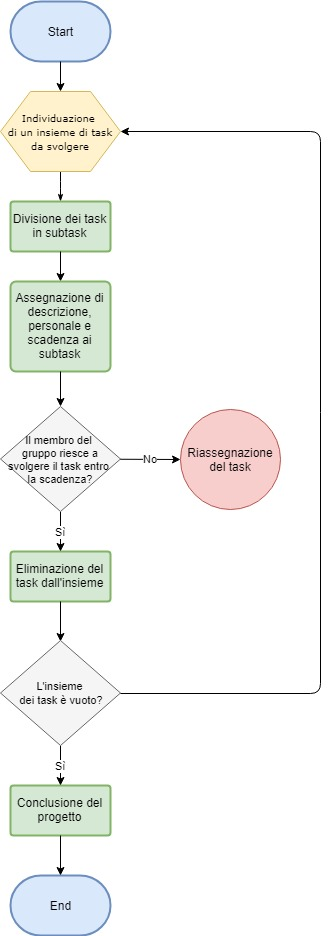
\includegraphics[scale=0.6]{ticketing}
		\centering
		\caption{Diagramma della procedura di individuazione e assegnazione dei task}
	\end{figure}
	
	\subsection{Gestione delle comunicazioni}
	
	\subsubsection{Comunicazioni interne}
	
	Le comunicazioni interne (ed alcune comunicazioni esterne con la Proponente compatibilmente con le sue necessità) avvengono tramite il tool di messaggistica multi-piattaforma con funzionalità specifiche per gruppi di lavoro \glossario{Slack}{Slack}. Tale strumento si integra con altre tecnologie selezionate dal gruppo offrendo la possibilità di ricevere notifiche riguardanti le modifiche della \glossario{repository}{Repository} \glossario{GitHub}{GitHub} o il progresso dei task assegnati con Wrike. Permette inoltre di creare canali tematici per rendere più efficiente lo scambio e il reperimento delle informazioni, nonché condividere file ed immagini utili allo sviluppo del progetto.
	\\ \noindent Per mantenere sotto continuo controllo l'avanzamento dei lavori è prevista, almeno una volta a settimana, una conversazione su \textit{Slack} in cui ogni membro del gruppo indica lo stato di avanzamento del \glossario{Task}{task} assegnatogli.
	\\ \noindent Per comunicazioni informali e per ricevere notifiche sommarie riguardanti le modifiche della \glossario{repository}{Repository} \glossario{GitHub}{GitHub} verrà usato un ulteriore tool di messaggistica, di nome \glossario{Telegram}{Telegram}.
	
	\subsubsection{Comunicazioni esterne}
	
	Il \textit{Responsabile del Progetto} è tenuto a mantenere le comunicazioni esterne utilizzando una cartella di posta elettronica appositamente creata:
	\[graphite.swe@gmail.com.\]
	Il \textit{Responsabile del Progetto} deve mantenere informati i restanti componenti del gruppo riguardo alle discussioni con terzi utilizzando i canali di comunicazione interna, ma per maggiore sicurezza ed evitare disguidi interni è previsto che alla ricezione di una mail sull'indirizzo di posta elettronica il messaggio venga inoltrato a tutti i componenti del gruppo.
	Compatibilmente con impegni e richieste della Proponente, alcune rapide comunicazioni esterne avverranno tramite canale dedicato Slack.
	
	\subsection{Gestione degli incontri}
	
	\subsubsection{Incontri interni}
	
	Il \textit{Responsabile di progetto} è incaricato di organizzare gli incontri interni dando comunicazione di data e ora tramite i canali di comunicazione. Inoltre deve essere comunicato prima di ogni riunione l'ordine del giorno sempre dal \textit{Responsabile di progetto}.
	\\ \noindent Per mantenere sotto continuo controllo l'avanzamento dei lavori è previsto almeno un incontro settimanale con l'intero gruppo.
	\\ \noindent Ogni componente del gruppo ha diritto di presentare una richiesta di organizzazione di un incontro al \textit{Responsabile di progetto} il quale può accogliere o meno la proposta.
	
	\subsubsection{Incontri esterni}
	
	Il \textit{Responsabile di Progetto} deve organizzare gli incontri esterni con il committente e comunicare al proprio gruppo data e ora in cui essi avvengono. Come per gli incontri interni, ogni componente del gruppo ha diritto ad una richiesta di organizzazione di un incontro esterno.
	\\ \noindent Per ogni incontro esterno deve essere preventivamente stilata una serie di domande tale da giustificare la richiesta di un appuntamento con il committente.
	
	\subsection{Gestione degli strumenti di versionamento}
	
	\subsubsection{Repository}
	
	Per il versionamento e il salvataggio dei file è previsto l'utilizzo di repository su GitHub. L'\textit{Amministratore di Progetto} si deve occupare della creazione delle repository e dell'aggiunta di tutti i componenti del gruppo, in possesso di un account personale, come collaboratori.
	\\ \noindent È previsto l'utilizzo di tre repository facenti capo all'account GitHub del gruppo Graphite:
	\begin{enumerate}
		\item Repository dedicata alla Documentazione;
		\item Repository dedicata al \textit{Proof of Concept} (e relativa pubblicazione);
		\item Repository dedicata al codice del prodotto.
	\end{enumerate}
	
	\subsubsection{Tipi di file e .gitignore}
	
	Nelle cartelle contenenti tutti i documenti saranno presenti solamente i file .tex, .pdf, .jpg, .png. Le estensioni dei file generati automaticamente dalla compilazione sosno stati aggiungi a .gitignore, e quindi vengono ignorati e resi invisibili a \glossario{Git}{Git}.
	
	\subsubsection{Norme sui commit}
	
	Ogni volta che vengono effettuate delle modifiche ai file del repository, le quali poi vengono caricate su di esso, bisogna specificarne le motivazioni. Questo avviene utilizzando il comando \textit{commit} accompagnato da un messaggio riassuntivo e una descrizione in cui va specificato: 
	\begin{itemize}
		\item la lista dei file coinvolti;
		\item la lista delle modifiche effettuate, ordinate per ogni singolo file.
	\end{itemize}

	\subsection{Gestione dei rischi}
	
	Il \textit{Responsabile di Progetto} ha il compito di rilevare i rischi indicati nel PP. Nel caso ne vengano individuati di nuovi dovrà aggiungerli nell'appendice dedicata dello stesso documento (§A "Esito della rilevazione dei rischi"). 
	\\ \noindent La procedura da seguire per la gestione dei rischi è la seguente:
	\begin{itemize}
		\item Registrazione di ogni riscontro dei rischi nel PP;
		\item Aggiunta dei nuovi rischi rilevati nell'appendice dedicata del PP;
		\item Individuazione di problemi non calcolati e monitoraggio di rischi già previsti;
		\item Ridefinizione, se necessaria, delle strategie di progetto.
	\end{itemize}
	
	\section{Miglioramento continuo}
	Il gruppo intende misurare, controllare, valutare e migliorare i processi a beneficio del ciclo di sviluppo del software, operando conformemente al principio del miglioramento continuo.
	
	\subsection{Costituzione dei processi}
	Per ogni processo stabilito, esso deve essere controllato, sviluppato e monitorato costantemente allo scopo di
	garantirne il raggiungimento degli obiettivi fissati nella pianificazione.
	
	\subsection{Valutazione dei processi}
	Allo scadere di ogni periodo pianificato, viene attivata una procedura di valutazione dei processi conformemente al ciclo \glossario{Ciclo di PDCA}{Ciclo di PDCA}. Per ogni processo viene valutato:
	\begin{itemize}
		\item Esito;
		\item Tempistiche;
		\item Inconvenienti;
		\item Metriche SPICE.
	\end{itemize}
	
	\subsection{Miglioramento dei processi}
	Giunti al periodo successivo, è necessario definire e applicare i miglioramenti necessari ed aggiornare la relativa documentazione.
	Dati storici, tecnici e di valutazione devono essere raccolti ed analizzati all'interno del PQ al fine di evidenziate eventuali punti deboli e le potenzialità dei processi impiegati. L'analisi
	è utilizzata come feedback per migliorare i processi e indicare modifiche da applicare in questo senso alle procedure, agli strumenti e alle tecnologie.
	
	\section{Formazione del personale}
	I membri del gruppo devono procedere autonomamente allo studio individuale del \textit{project management} e delle tecnologie che verranno utilizzate nel corso del progetto, riferendosi a:
	\begin{itemize}
		\item Materiale elencato nella sezione "Riferimenti informativi" di ogni documento;
		\item Siti web e relativa documentazione delle tecnologie riportati in forma di link in §4.6 di questo documento;
		\item Membri del gruppo più esperti;
		\item Seminario su CMAKE offerto dalla Proponente e reperibile al seguente link:
		\begin{center}
			\url{https://github.com/giuliopaci/cmake-tutorial}
		\end{center} 
	\end{itemize}
	Occorre stabilire e fornire in tempo l'adeguata preparazione in termini di sviluppo di competenze e conoscenze richieste. Il personale dove essere formato preventivamente alla pianificazione fissata, in modo da poter svolgere adeguatamente i compiti
	assegnati. Qualora alcuni membri non riescano a colmare determinate lacune, essi devono informare al più presto il \textit{Responsabile di Progetto} che provvede a redistribuire i compiti assegnati o a indicare materiale utile allo sviluppo delle competenze/conoscenze necessarie allo svolgimento del task.
	Il versionamento dei prodotti viene usato anche come strumento per apprendere dall'operato altrui, così da integrare le conoscenze personali migliorando la qualità e l'efficienza delle attività di formazione.
	
	\section{Strumenti}
	
	\subsection{Organizzazione}
	
	\subsubsection{Sistema operativo}
	
	Il gruppo di progetto lavora sui seguenti sistemi operativi:
	\begin{itemize}
		\item Ubuntu 17.10 x64;
		\item Ubuntu 16.04 \glossario{LTS}{LTS} x64;
		\item Windows 10 Home x64;
		\item Windows 10 Pro x64;
		\item Windows 7 Home Premium.
	\end{itemize}

	\subsubsection{Google Drive}
	Google Drive è un servizio di memorizzazione e sincronizzazione online introdotto da Google. Il servizio comprende il file hosting, il file sharing e la modifica collaborativa di documenti fino a 15 GB gratuiti ed è perfettamente integrato con altri servizi Google quali Gmail, Docs, Sheets, Slides e Forms. Il gruppo intende utilizzare Drive per il rilascio della documentazione prevista per le revisioni di progetto e per il salvataggio di materiale informale che possa necessitare di elaborazione collaborativa. Il servizio prevede un piano gratuito automaticamente associato alla creazione di un account Google, ed è reperibile al seguente link:
	\begin{center}
		\url{https://www.google.com/intl/it_ALL/drive/using-drive/}
	\end{center}
	
	\subsubsection{Hangouts}
	Hangouts è un software di messaggistica istantanea e di VoIP sviluppato da Google. È disponibile per le maggiori piattaforme mobili e come estensione per il browser web Google Chrome, e si integra perfettamente con l'ecosistema di prodottoti Google. Il gruppo intende utilizzare tale tecnologia per effettuare videochiamate tra i membri e/o con la Proponente (caso in cui il contatto in remoto si è rivelato indispensabile a causa degli obblighi logistici della stessa) nel contesto di riunioni e confronti. La tecnologia è gratuita sia in versione mobile che desktop, maggiori informazioni sono reperibili al seguente link:
	\begin{center}
		\url{https://gsuite.google.it/learning-center/products/hangouts/get-started/}
	\end{center}
	
	\subsubsection{Slack}
	
	\textit{Slack} è uno strumento di collaborazione aziendale utilizzato particolarmente per lo scambio di messaggi tra componenti di un team. L'idea di partenza di questo software è di essere un totale rimpiazzo degli scambi di E-mail e sms ma a questo si aggiunge la possibilità di aggiungere plugin per la notifica di attività annesse al proprio ambiente di lavoro.
	\\ \noindent Verranno in particolare sfruttati i plugin per la notifica di attività sulla repository e per discussioni riguardo ai task presenti sulla piattaforma Wrike. La tecnologia offre un piano gratuito che non limita il gruppo entro i confini degli obiettivi di progetto, ed è accessibile al seguente link:
	\begin{center}
		\url{https://slack.com/features}
	\end{center}
	
	\subsubsection{Telegram}
	
	\textit{Telegram} è una applicazione di messaggistica nata come applicazione mobile e successivamente portata anche su Windows, Mac e varie distribuzioni Linux. Rispetto agli altri sistemi di messaggistica \textit{Telegram} consente un facile passaggio di immagini e documenti in più formati mantenendo inoltre nel proprio cloud storage tali file per un agevole recupero su qualsiasi dispositivo. È possibile creare gruppi di utenti la cui chat ha soprattutto il valore aggiunto di poter contenere sistemi automatici per l'organizzazione di sondaggi e la comunicazione di messaggi importanti da tenere in sovrimpressione. Telegram è accessibile gratuitamente al seguente link:
	\begin{center}
		\url{https://telegram.org/}
	\end{center}
	
	\subsubsection{Wrike}
	
	\textit{Wrike} è un' applicazione web disponibile anche per dispositivi mobile creata per aiutare i team a tracciare il proprio lavoro. Le sue principali funzionalità si dividono in:
	\begin{itemize}
		\item possibilità di creare dei task, assegnarvi delle persone, darne una priorità e controllarne lo stato di completamento;
		\item capacità di creare in modo automatico diagrammi di Gantt basati sui task inseriti dall'utente;
		\item possibilità di condivisione file con la possibilità di farci delle modifiche online;
		\item possibilità di creazione di resoconti e discussioni riguardo a specifici argomenti;
		\item servizio di notifica e modifica rapida tramite l'applicazione per dispositivi mobile.
	\end{itemize}
	
	Il gruppo intende fare di Wrike il principale strumento a supporto del \textit{project management} e quindi utilizzarlo per la suddivisione e assegnazione del lavoro in task da parte del \textit{Responsabile}, sfruttando nel contempo le altre sue funzionalità per documentare e monitorare la gestione di progetto. Pur essendo uno strumento prettamente commerciale, Wrike è disponibile gratuitamente per gli studenti al seguente link:
	\begin{center}
		\url{https://www.wrike.com/it/tour/}
	\end{center}
	
	\subsubsection{Git}
	
	\textit{Git} è un software di controllo versione distribuito utilizzabile da interfaccia a riga di comando. Pensato per mantenere un grande progetto di sviluppo distribuito, Git supporta fortemente lo sviluppo non lineare del software.
	\\ \noindent Tramite strumenti appositi è possibile creare più diramazioni di sviluppo del software con la garanzia di poter mantenere in locale la cronologia di sviluppo completa.
	\\ \noindent In sostituzione ai comandi testuali molti membri del gruppo utilizzeranno \glossario{Gitkraken}{Gitkraken} o \textit{GitHub Desktop} come interfaccia grafica per la gestione della repository. La tecnologia è open source e reperibile gratuitamente al seguente link:
	\begin{center}
		\url{https://git-scm.com/about}
	\end{center}
	
	\subsubsection{GitHub}
	
	GitHub è un servizio di \glossario{hosting}{hosting} per progetti software. Il sito è principalmente utilizzato dagli sviluppatori, che caricano il codice sorgente dei loro programmi e lo rendono scaricabile dagli utenti. Può essere utilizzato anche per la condivisione e la modifica di file di testo e documenti revisionabili.
	\\ \noindent Un utente può interagire con lo sviluppatore tramite un sistema di issue tracking, pull request e commenti che permette di migliorare il codice della repository, risolvendo bug o aggiungendo funzionalità. Lo strumento è reperibile gratuitamente al seguente link:
	\begin{center}
		\url{https://github.com/features}
	\end{center}
	
	% DOCUMENTAZIONE
	
	\subsection{Documentazione}
	
	Per redarre la documentazione, il gruppo utilizza i seguenti strumenti:
	
	\subsubsection{LaTex}
	\LaTeX è un linguaggio di markup, usato per la preparazione di testi, basato sul programma di composizione tipografica TEX. Il gruppo intende utilizzare tale tecnologia per la produzione collaborativa della documentazione formale, in particolare attraverso lo stumento \textit{TeXstudio}. La tecnologia è reperibile gratuitamente al seguente link:
	\begin{center}
		\url{https://www.latex-project.org/}
	\end{center}
		
	\subsubsection{TexStudio}
	TexStudio è un IDE per \LaTeX che il gruppo utilizza per la stesura della documentazione in virtù delle innumerevoli funzionalità che offre gratuitamente e del fatto che si tratta di un'applicazione cross-platform supportata dai maggiori sistemi operativi. Lo strumento è reperibile gratuitamente al seguente link:
	\begin{center}
		\url{https://www.texstudio.org/}
	\end{center}
		
	\subsubsection{SWEgo} Il tracciamento dei requisiti e dei casi d'uso viene effettuato tramite il software \glossario{SWEgo}{SWEgo} e successivamente controllato manualmente per assicurarne la correttezza. Lo strumento è accessibile gratuitamente al seguente link:
	\begin{center}
		\url{http://www.swego.it/}
	\end{center}
		
	\subsubsection{LucidChart}
	Per la produzione di diagrammi UML viene utilizzato il software gratuito \glossario{Lucidchart}{Lucidchart}. Lo strumento è accessibile gratuitamente al seguente link:
	\begin{center}
		\url{https://www.lucidchart.com/pages/tour}
	\end{center}

	% SVILUPPO

	\subsection{Sviluppo}

	Per lo sviluppo software relativo al progetto, il gruppo utilizza i seguenti strumenti:
	
	\subsubsection{Sistema operativo di riferimento}
	Ubuntu è un sistema operativo focalizzato sulla facilità di utilizzo. È prevalentemente composto da software libero proveniente dal ramo instabile di Debian GNU/Linux, ma contiene anche software proprietario, ed è distribuito liberamente con licenza GNU GPL. È orientato all'utilizzo sui computer desktop, ma presenta delle varianti per altri dispositivi, ponendo grande attenzione al supporto hardware. Il gruppo intende utilizzare Ubuntu v16.04 LTS come sistema operativo di riferimento per lo sviluppo del prodotto, offrendone garanzia di corretto funzionamento sullo stesso. Ubuntu è reperibile al seguente link:
	\begin{center}
		\url{https://www.ubuntu-it.org/progetto}
	\end{center}
	
	\subsubsection{Libreria di riferimento}
	Speect è un sistema di \textit{Text To Speech} (TTS) multilingua. Esso offre un sistema TTS completo (analisi e decodifica del testo e sintesi vocale) con annesse varie API, nonché un ambiente per la ricerca e lo sviluppo di sistemi e voci TTS. Speect è scritto in linguaggio C, con una stretta conformità allo standard ISO / IEC 9899: 1990, consentendo così la massima portabilità su diverse piattaforme di calcolo. Le chiamate di sistema specifiche della piattaforma sono astratte per consentire le porte a nuove piattaforme. Speect v1.1.0-69-g65f4 rappresenta il cuore del prodotto che il gruppo intende sviluppare ed in particolare è l'applicazione per la quale si vuole realizzare un'interfaccia grafica atta a semplificarne l'utilizzo e il debug. La tecnologia è open source e la sua documentazione è accessibile al seguente link:
	\begin{center}
		\url{http://speect.sourceforge.net/contents.html}
	\end{center}

	\subsubsection{IDE}

	QT è una libreria multipiattaforma per lo sviluppo di programmi con interfaccia grafica tramite l'uso di widget (congegni o elementi grafici). La libreria è scritta in C++ e gode di ampia diffusione e supporto. Il gruppo intende utilizzare questa tecnologia nella versione v5.9 LTS per lo sviluppo dell'interfaccia grafica del prodotto. Qt è reperibile al seguente link:
	\begin{center}
		\centerline{\url{https://www.qt.io/what-is-qt/}}
	\end{center}

	\subsubsection{Compilazione}

	Per la compilazione vengono utilizzati i seguenti strumenti:

	\begin{itemize}
		\item \textbf{GCC}: il compilatore che verrà usato per la compilazione del software è il \glossario{GCC}{GCC} (GNU Compiler Collection). Il compilatore è reperibile al seguente link:
		\begin{center}
			\centerline{\url{https://gcc.gnu.org/}}
		\end{center}
	
		\item \textbf{Cmake}: CMake è una famiglia di strumenti open source e multipiattaforma progettati per creare, testare e pacchettizzare software. CMake viene utilizzato per controllare il processo di compilazione del software utilizzando semplici file di configurazione indipendenti dalla piattaforma e dal compilatore e generare makefile e aree di lavoro nativi che possono essere utilizzati nell'ambiente del compilatore di propria scelta. Il gruppo intende utilizzare questa tecnologia nella versione v3.10.2 per l’automazione della compilazione del prodotto. Lo strumento è reperibile al seguente link:
		\begin{center}
			\centerline{\url{https://cmake.org/overview/}}
		\end{center}
	
	\end{itemize}

	\subsubsection{GUI}

	Per progettare l'interfaccia grafica viene utilizzato \glossario{Qt Creator}{Qt Creator}. Questo strumento permette di realizzare interfacce grafiche mediante le librerie grafiche Qt, diventate in questo ambito quasi uno standard per piattaforme Linux Based. Qt Creator è disponibile al seguente link: 
	\begin{center}
		\centerline{\url{https://www.qt.io/qt-features-libraries-apis-tools-and-ide/}}
	\end{center}
	
	% VERIFICA
	
	\subsection{Verifica}
	
	\subsubsection{Verifica della documentazione}
	
	\begin{itemize}
		\item \textbf{Verifica ortografica:} Per eseguire controlli ortografici sulla documentazione viene utilizzata la verifica dell’ortografia in tempo reale, strumento integrato in TexStudio che sottolinea in rosso le parole errate secondo la lingua italiana;
		
		\item \textbf{Verifica della leggibilità:} Per calcolare l'\glossario{indice Gulpease}{indice Gulpease} a verifica della leggibilità dei documenti viene utilizzato uno script apposito reperibile al link seguente:
		\begin{center}
			\centerline{\url{https://github.com/LeafSWE/Leaf/tree/master/Documents/Gulpease}}
		\end{center}
	\end{itemize}
	
	\subsubsection{Verifica del software}
	
	\begin{itemize}
		\item \textbf{Test:} Google Test è un framework per la realizzazione di test per il linguaggio C++. Il gruppo intende utilizzare questa tecnologia per la realizzazione dei test del software, ulteriori informazioni sono reperibili al seguente link:
		\begin{center}
			\url{https://github.com/google/googletest/blob/master/googletest/docs/Primer.md}
		\end{center}
		\item \textbf{Testing Automatico:} Travis CI è un servizio di integrazione continua distribuito utilizzato per costruire e testare progetti software ospitati su GitHub. I progetti open source possono essere testati gratuitamente attraverso il sito web \url{travis-ci.org}. Il gruppo intende utilizzare questa tecnologia per l'esecuzione di test automatici a seguito del caricamento di codice sulla repository relativa al progetto, così da garantirne la correttezza. Travis CI è accessibile al seguente link:
		\begin{center}
			\url{https://docs.travis-ci.com/}
		\end{center}
		
		\item \textbf{Analisi statica:} Per l’analisi statica del codice viene usato il software \glossario{Valgrind}{Valgrind}. La \glossario{suite}{suite} di strumenti Valgrind fornisce numerosi strumenti di \glossario{debugging}{debugging} e di \glossario{profiling}{profiling} che aiutano a rendere i programmi più performanti e più corretti. Il più popolare di questi strumenti è chiamato Memcheck, ed è in grado di rilevare molti errori relativi alla memoria comuni nei programmi C e C++ e che possono causare arresti anomali e comportamenti imprevedibili. Valgrind è accessibile al seguente link: 
		\begin{center}
			\url{http://valgrind.org/}
		\end{center}
		
		\item \textbf{Analisi dinamica:} Per l’esecuzione dei test di analisi dinamica viene usato il software \glossario{SonarQube}{SonarQube}, una piattaforma open source per la gestione della qualità del codice. SonarQube è un’applicazione web che produce report sul codice duplicato, sugli standard di programmazione, i test di unità, il \glossario{code coverage}{code coverage}, la complessità, i bug potenziali, i commenti, la progettazione e l’architettura. SonarQube è accessibile al seguente link:
		\begin{center}
			\url{https://www.sonarqube.org/}
		\end{center}
		
		\item \textbf{Metriche legate al software:} Per il controllo delle varie metriche vengono utilizzati i software:
		\begin{itemize}
			\item \textbf{Better Code Hub}: \glossario{Better Code Hub}{Better Code Hub} è un servizio di analisi del codice sorgente web-based che controlla il codice per la conformità rispetto a 10 linee guida per l'ingegneria del software e fornisce un \glossario{feedback}{feedback} immediato per capire dove concentrarsi per miglioramenti di qualità. Better Code Hub è accessibile al seguente link:
			\begin{center}
				\url{https://bettercodehub.com/}
			\end{center}
		
			\item \textbf{Codacy}: Codacy è uno strumento di analisi / qualità del codice automatizzato, con cui si ottengono analisi statiche, complessità ciclomatica, indicazioni sulla duplicazione e le variazioni della copertura dei test dell'unità di codice in ogni richiesta di commit e pull. È inoltre possibile utilizzare Codacy per applicare uno standard di qualità del codice e applicare le best practice sulla sicurezza, il tutto integrato con GitHub. Ulteriori informazioni su Codacy sono disponibili al seguente link:
			\begin{center}
				\url{https://www.codacy.com/features}
			\end{center}
		\end{itemize} 
	\end{itemize}

	
	\subsection{Schema riepilogativo dell'interazione \\ delle tecnologie e degli strumenti}
	
	Segue uno schema che riassume l'interazione e l'uso delle tecnologie e degli strumenti selezionati.
	
	\begin{figure}
		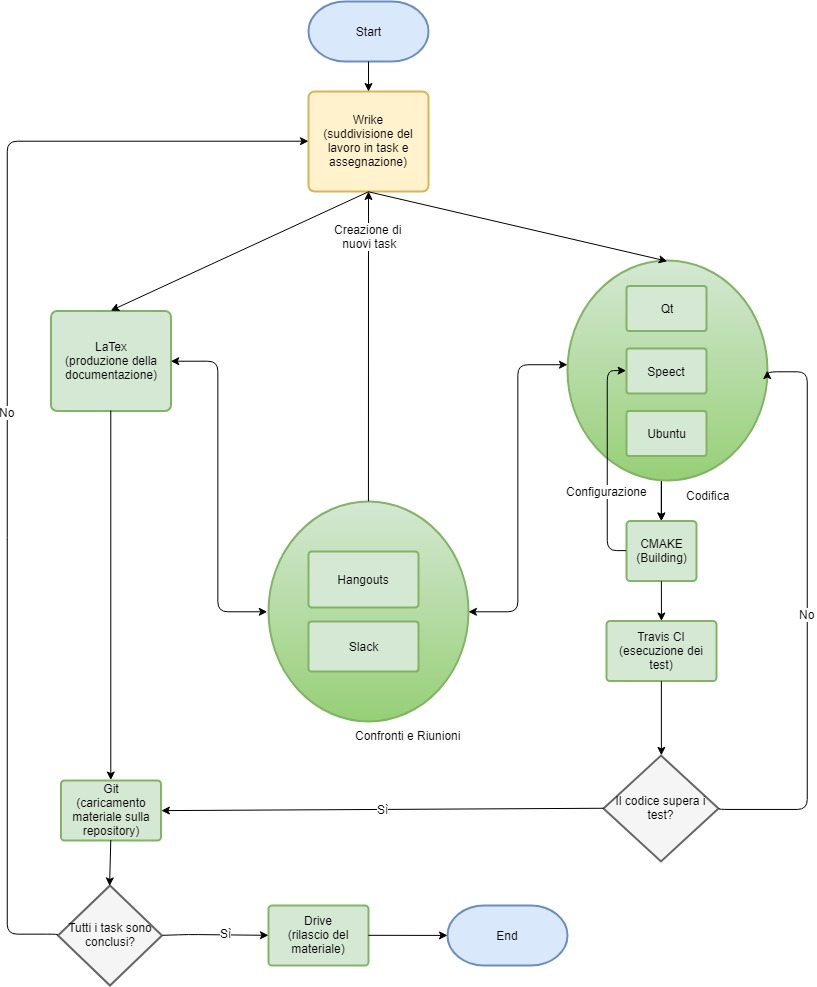
\includegraphics[scale=0.5]{tech-integration}
		\centering
		\caption{Schema riepilogativo dell'interazione delle tecnologie}
	\end{figure}
\end{document}